\chapter{TF-IDF Shortfalls}
\label{ch:tfidfshortfalls}

As mentioned previously, the need for text preprocessing is eminent, but we must use better tools to avoid destroying the context and patterns offered by natural speech. Furthermore, using PCA isn't as helpful when not dealing with numerical attributes but rather large vectors of text embeddings.

\begin{figure}
  \centering
  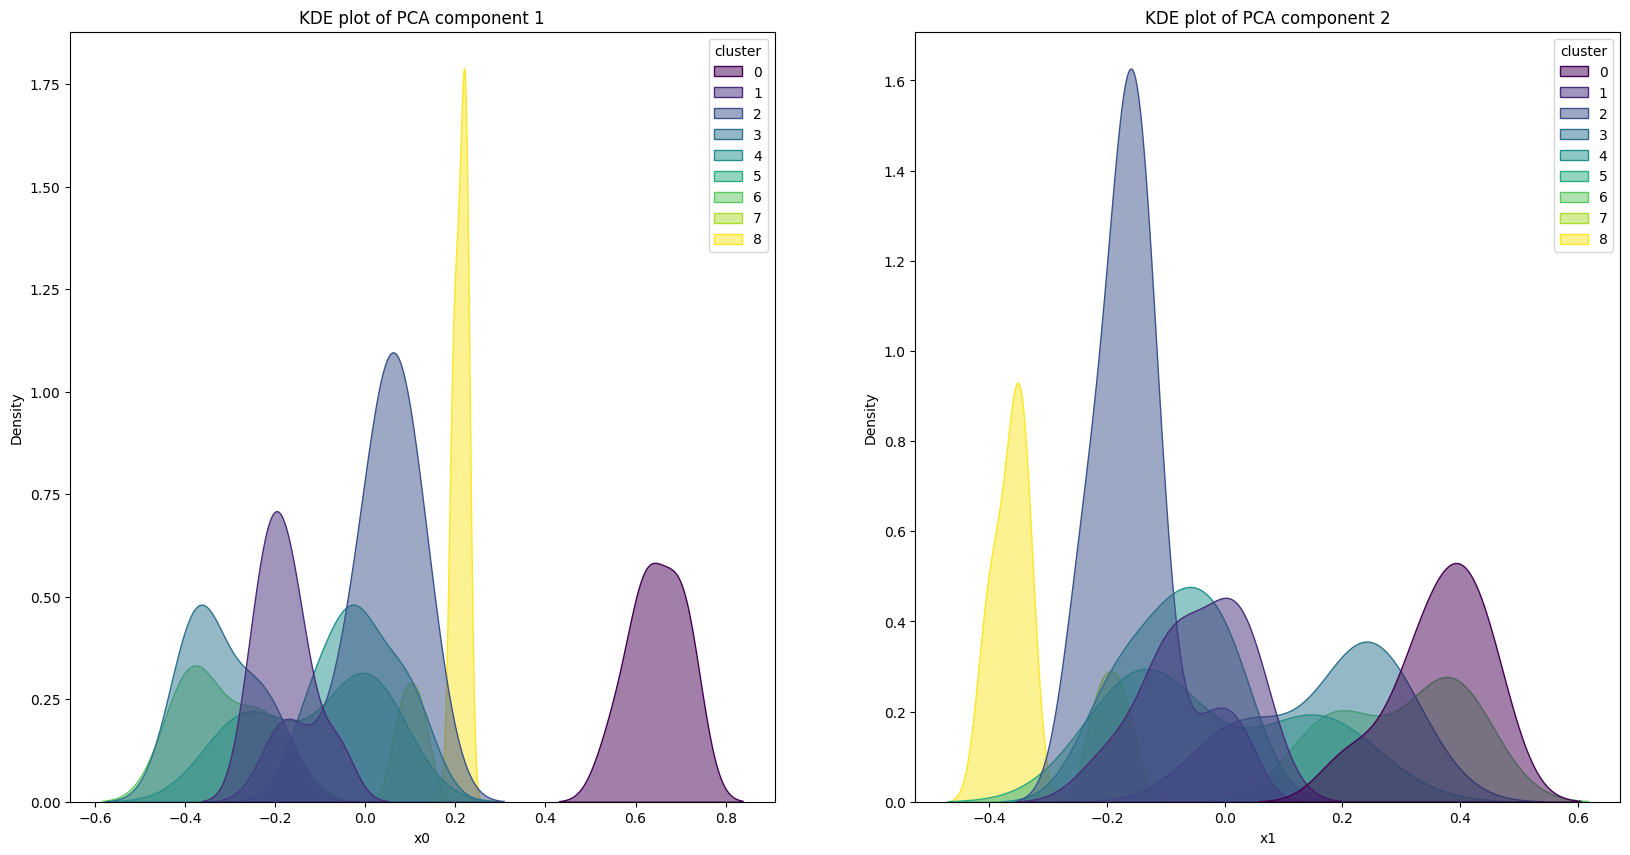
\includegraphics[width=0.9\textwidth]{kde_tfidf}
  \caption{KDE Plot of TF-IDF PCA Components}
  \label{fig:tfidf_kde}
\end{figure}

If we analyze the KDE plots (Figure ~\ref{fig:tfidf_kde})) of each PCA component, we can see that our module distribution is not as chaotic as it seemed from the scatterplot. We can observe that the higher the density peak and the skinnier the density bell is of a given cluster, the more closely we were able to associate them using document embeddings and PCA feature scaling.

\begin{figure}
  \centering
  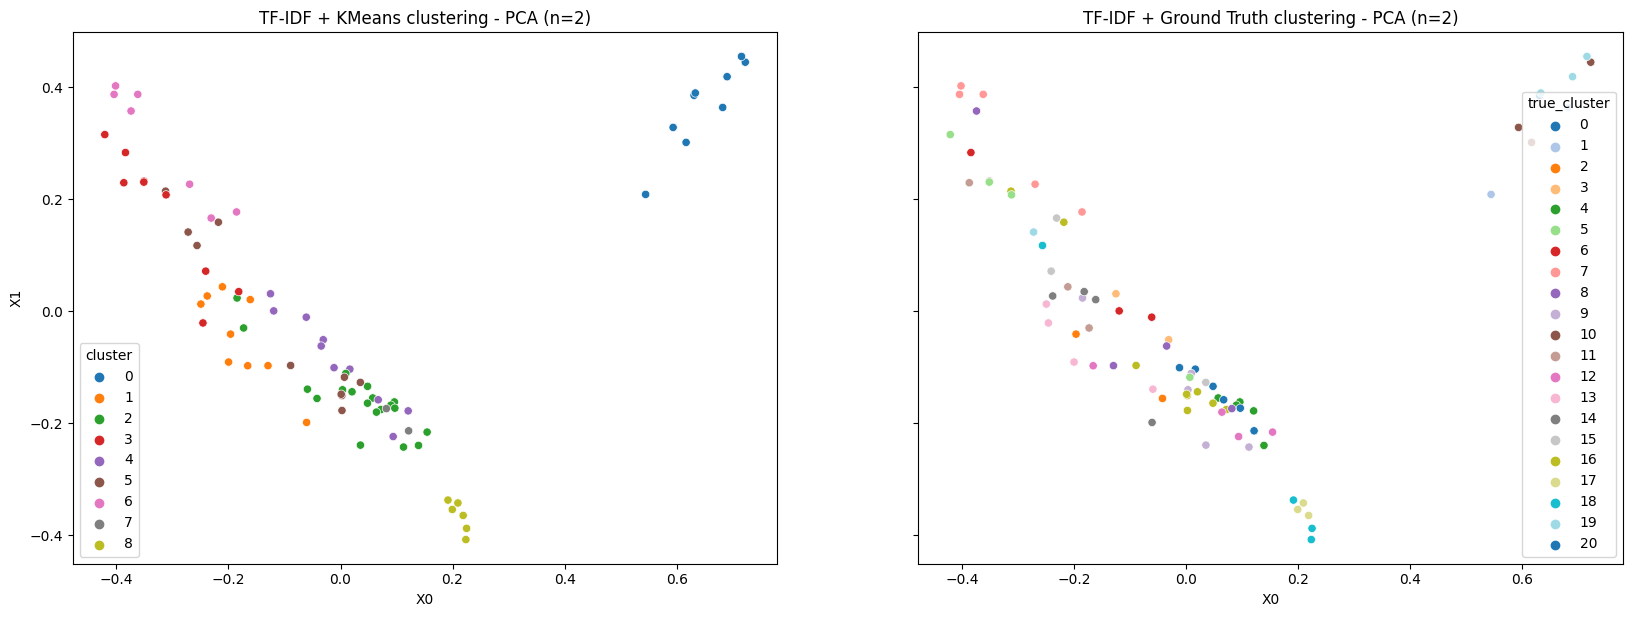
\includegraphics[width=0.9\textwidth]{short_scatter}
  \caption{Scatterplot of TF-IDF PCA Components}
  \label{fig:tfidf_scatter}
\end{figure}

When looking to validate the clustering algorithm, we can turn our attention to the second scatterplot on the right, which differentiates between marks using their ground truth cluster. From this (Figure ~\ref{fig:tfidf_scatter}), we can observe that, for example, "true cluster" numbers 18 and 17 are very close on the plot meaning they both cover relatively the same concepts, as interpreted by TF-IDF. Due to this, the K-Means algorithm clustered them together, making cluster number 8 in the process.
